\chapter{From T1 images to numerical simulation}
\label{chp:chp3}

The goal of this chapter is to enable numerical simulation over a
brain region defined from structural MR images. To address this
challenge, we first demonstrate how to generate a high quality mesh of
a brain hemisphere from T1-weighted MR images using the tools
introduced in Chapter~\ref{chp:chp2}. Next, we show how to define a
finite element discretization of the diffusion
equation~\eqref{eq:diffusion} over this mesh to simulate the influx of
an injected tracer.

\section{Generating a volume mesh from T1-weighted MRI}
\label{sec:chp3:tools}

To generate a mesh from an MRI data set including T1-weighted images,
we follow three main steps:
\begin{enumerate}
\item
  Extract a T1-weighted image series from the MRI dataset,
\item
  Create (boundary) surfaces from the T1-weighted images using FreeSurfer,
\item
  Generate a volume mesh of the interior using FreeSurfer along with \svmtk.
\end{enumerate}
We will consider each of these steps in order and encourage the
reader to ensure that FreeSurfer is installed and configured (see
Chapter~\ref{sec:chp2:tools:freesurfer}) before proceeding. Step 2 can
be particularly time consuming, likely with FreeSurfer segmentation
and reconstruction run times of up to 24 hours.
While we provide already processed files in the tarball that accompanies
the book, we encourage the reader to try these steps.
 
\subsection{Extracting a single series from an MRI dataset}

\index{DicomBrowser}
To extract a single MR series from an MRI dataset or a DICOM database,
we can use the DicomBrowser graphical interface or FreeSurfer command
line tools. The first option, using the DicomBrowser graphical
interface to extract a T1-weighted image series, is described in
Chapter~\ref{sec:chp2:viewmri} with the book data set as an example,
and the resulting image series can be found under \ernieT1 in
the book data set. The second option is described in
Chapter~\ref{sec:chp3:advanced} at the end of this chapter.

\subsection{Creating surfaces from T1-weighted MRI}
\label{sec:chp3:surfaces}

\index{FreeSurfer}
\index{FreeSurfer!\emp{recon-all}}
\index{MRI!T1}

The next step is to create surfaces, representing, for example, the
interface between the pial membrane and the surrounding cerebrospinal
fluid (CSF), referred to here as the pial surface, or the interface
between white and gray matter, from the T1-weighted MRI series just
extracted. We will use FreeSurfer for this task, and as an example, we
will extract the pial surface surrounding the left hemisphere of a
brain.

To conduct a full image stack segmentation and surface reconstruction,
we take advantage of the FreeSurfer command \emp{recon-all}. This
command is compute-intensive, with run times likely up to 24
hours. To invoke \emp{recon-all}, we select one of the T1 DICOM files:
for instance, in~\emp{\ernieT1}, we can pick \emp{IM\_0162}. Next, we
decide on a subject identifier for the FreeSurfer pipeline; we choose
to name this example subject ernie. We are now ready to launch
\emp{recon-all}\footnote{This is a good thing to do on a separate
  core or overnight.}

\terminal{\$ cd \emp{\ernieT1} \\
  \$ recon-all -subjid ernie -i IM\_0162 -all}

The results of \emp{recon-all} will be output to the folder
\emp{SUBJECTS\_DIR/ernie}, where the environment variable
\emp{SUBJECTS\_DIR} defaults to the \emp{subjects} folder under
\emp{FREESURFER\_HOME} (see
Chapter~\ref{sec:chp2:tools:freesurfer}). For convenience, this output
is also included in the book data set, under \emp{\ernieoutput}. If we
inspect the contents of this directory we will see several
subdirectories. Some important subdirectories are
\begin{itemize}
\item \emp{/stats}, contains files providing statistics derived during segmentation;
\item \emp{/mri}, contains volume files generated during segmentation; and
\item \emp{/surf}, contains surface files generated during segmentation.
\end{itemize}

%
\index{Freeview}
%
To view the generated surface files, we focus on the \emp{/surf}
directory, and launch Freeview (see
Chapter~\ref{sec:chp2:tools:freesurfer}):
\terminal{\$ cd \ernieoutput/surf\\
\$ freeview \&}
\noindent Targeting the pial surface that surrounds the left brain
hemisphere as an example, select \button{File$\rightarrow$Load Surface}
from the command bar, and then select the file titled \emp{lh.pial}
(where \emp{lh} refers to left hemisphere and \emp{pial} denotes the pial
surface). After a moment, the view windows will be populated with 2D
surface slices shown as curves, in addition to a reconstructed 3D
image of the pial surface (Figure~\ref{fig:chp3:freeview-scr}).
\begin{figure}%\sidecaption
  \centering
  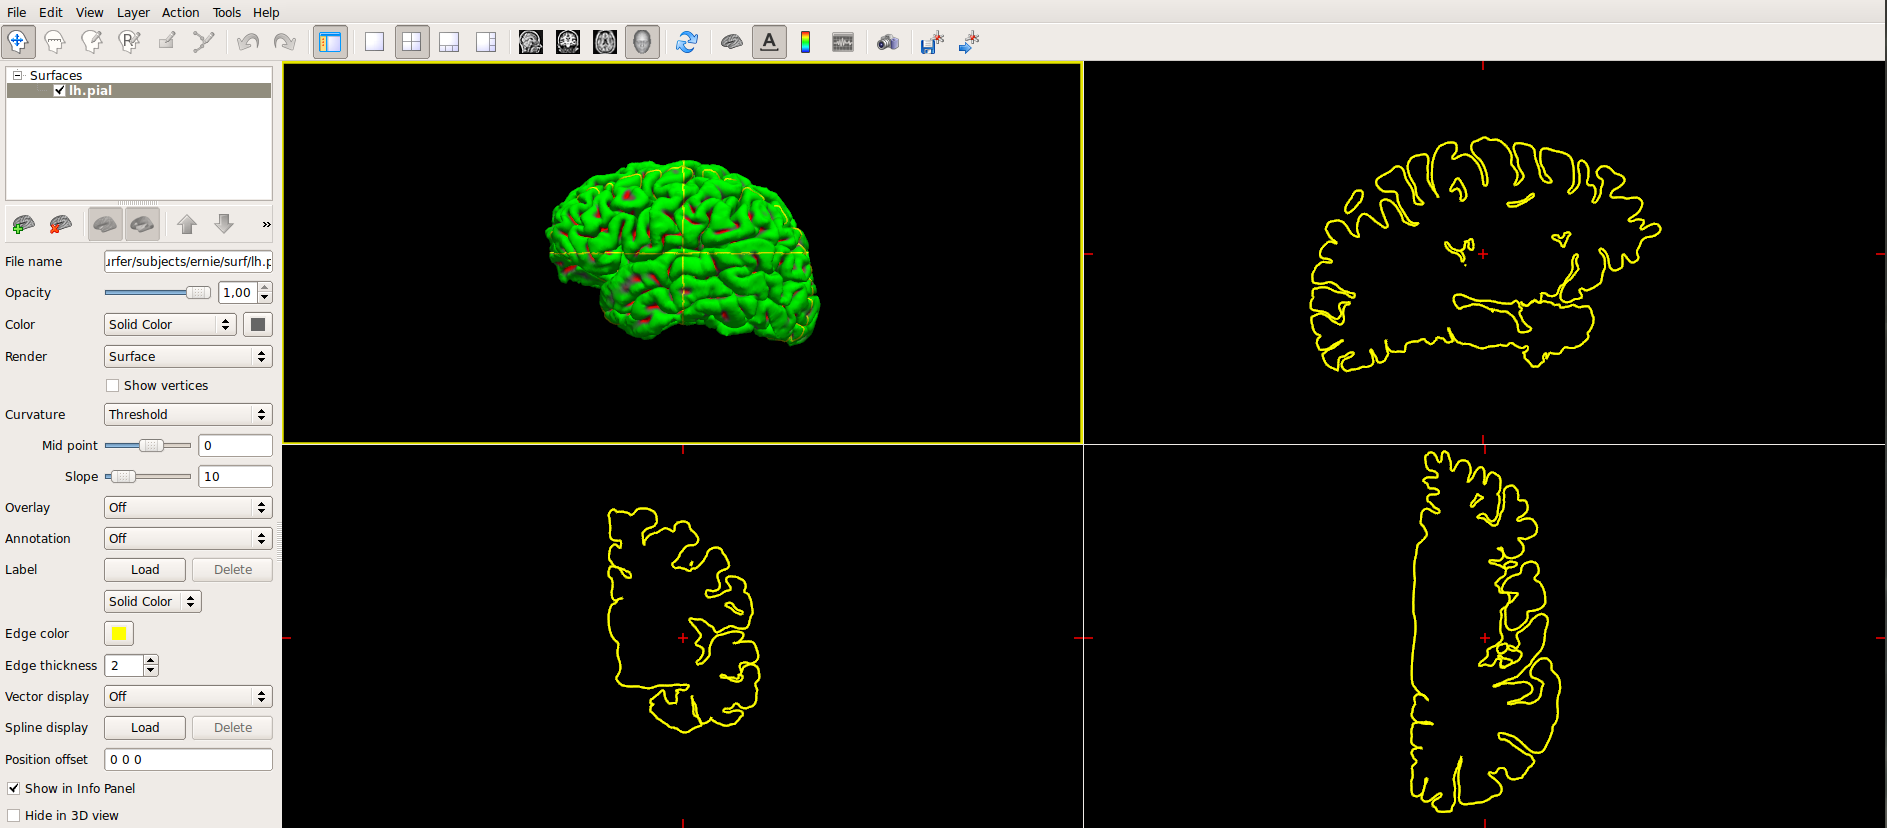
\includegraphics[width=0.95\textwidth]{./graphics/chp3/freeviewexscr}
  \caption{Freeview visualization of the pial surface of a single
    brain hemisphere extracted from T1 images via FreeSurfer.}
  \label{fig:chp3:freeview-scr}
\end{figure}

%
\index{FreeSurfer!\emp{mris\_convert}}
%\index{STL}
%\index{ParaView}
%
To work further with this surface, we use the FreeSurfer tool
\emp{mris\_convert} to convert the binary surface file into the STL
format~\cite{roscoe1988stereolithography}. STL is a widely used format
representing the surface discretely in terms of vertices, triangles
and normals. Generally, \emp{mris\_convert} is used to handle the
conversion between different surface formats. For instance, in the
directory \emp{\ernieoutput/surf}, we can run

\terminal{\$ mris\_convert ./lh.pial pial.stl}

\noindent to create the file \emp{lh.pial.stl} in the current
directory. The resulting file can be opened in several different
programs, for instance, ParaView or Gmsh.

\subsection{Creating a volume mesh from a surface}
\label{subsec:chp3:mesh-creation}

%
\index{mesh generation}
\index{SVM-Tk}
\index{SVM-Tk!\emp{Domain}}
\index{SVM-Tk!\emp{Surface}}
\index{SVM-Tk!\emp{create\_mesh}}
\index{SVM-Tk!\emp{save}}
%
The third step of our initial meshing pipeline is to generate a mesh
of the volume bounded by the surface representation. We will use the
tailored package \svmtk{} (see
Chapter~\ref{sec:chp2:tools:meshing:svmtk}) to convert from the STL
surface representation to a volume mesh. The Python script below (
\emp{mri2fem/chp3/surface\_to\_mesh.py} in the book scripts)
demonstrates the fundamentals of this process. The script (and all
similar scripts in the following) can then be run from there as
\terminal{\$ python surface\_to\_mesh.py}
Recall that Python version 3 is required.  If you have more than one version 
of python installed on your machine you may need to use `python3' in the 
above, and all further commands, instead of the `python' directive; this will 
explicitly specify which version of Python should be used to execute the 
script at hand.  %
%
The script \pythoninline{surface\_to\_mesh.py} defines a Python function, 
named \pythoninline{create\_volume\_mesh}, within it that can be called as
\newpythonsnippet{chp3}{surface_to_mesh.py}{15}{16}

\noindent The function itself reads
\newpythonsnippet{chp3}{surface_to_mesh.py}{0}{12}

\noindent Given an input STL filename (\pythoninline{stlfile}), an
output mesh filename with the \pythoninline{mesh} suffix
(\pythoninline{meshfile}), and an optional mesh resolution
(\pythoninline{resolution}, defaulting to 16), the script creates an
\svmtk{} \pythoninline{Domain} object, generates a volume mesh from the
surface via the call to \pythoninline{create\_mesh}, and saves this
mesh in the \pythoninline{.mesh} format to the output mesh file. The
mesh resolution parameter determines the maximum size of a tetrahedron
in the volume mesh (relative to the overall bounding box length for
the input surface): the higher the value, the higher the resolution,
that is, the smaller the volume of each element in the volume mesh
generated. Figure \ref{fig:chp3:ernie-volume-mesh} shows meshes with
\pythoninline{resolution = 16} (left) and \pythoninline{resolution =
  64} (right). Mesh generation can be a costly operation, with higher
run times (on the order of seconds to minutes) for higher resolutions.
\begin{figure}
  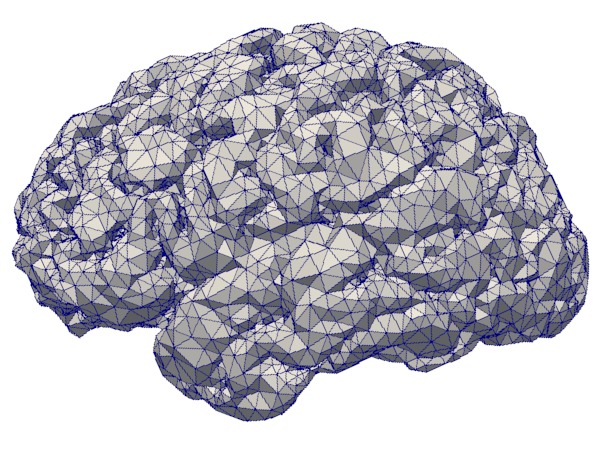
\includegraphics[width=0.49\textwidth]{./graphics/chp3/ernie-volume-16-r.png}
  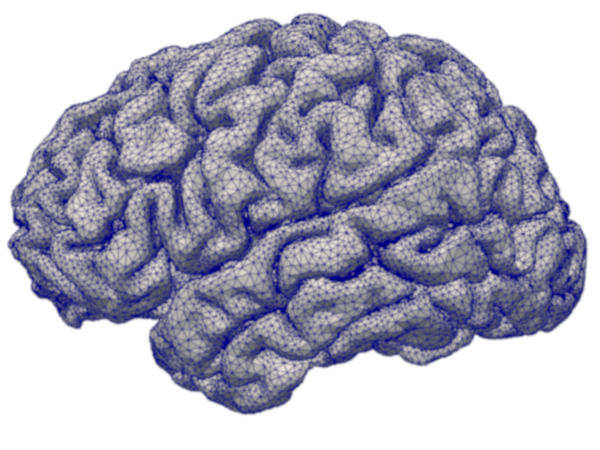
\includegraphics[width=0.49\textwidth]{./graphics/chp3/ernie-volume-64-r.png}
  \caption{Volume meshes of a left brain hemisphere produced by
    {\svmtk} from STL surface files, with lower (left) and higher
    (right) mesh resolutions.}
  \label{fig:chp3:ernie-volume-mesh}
\end{figure}

\index{meshio}
\index{ParaView}
The \emp{.mesh} format is the standard mesh format for \svmtk{} and
CGAL. However, it is not native to \fenics{}, and we therefore need to
convert the mesh to a \fenics-supported file format (for example .xml, .xdmf,
.h5). The Python package meshio (see~Chapter
\ref{sec:chp2:meshio}) is well suited for this purpose and can
convert between many different input and output mesh formats. For
instance, to convert to the FEniCS .xdmf format, we can run
\terminal{\$ meshio-convert lh.mesh lh.xdmf}
\noindent The .xdmf file can then be viewed in, for example, ParaView.

\section{Improved volume meshing by surface preprocessing}
\label{sec:chp3:improved-volume-meshing}
In the previous section, we stepped through the main pipeline for
generating a volume mesh from MR images. However, the brain surfaces
generated from T1 images often have a number of weaknesses:
\begin{itemize}
\item The surfaces can have unphysiologically sharp corners,   
\item The surfaces can include triangles with very large aspect ratios, 
\item The surfaces can have topological defects such as holes, and
\item The surfaces can self-intersect or overlap with other surfaces.   
\end{itemize}
These defects can cause the volume mesh generation to fail or result
in low-quality meshes that are not suitable for numerical
simulation. Therefore, surface preprocessing is often required to
enhance surface quality prior to generating volumetric meshes. Here,
we outline three main aspects of surface preprocessing: remeshing,
smoothing and separation. The enhanced STL surfaces can then be
directly inserted into the volume mesh generation described above in
Chapter~\ref{subsec:chp3:mesh-creation}.

\subsection{Remeshing a surface}
\label{subsubsec:chp3:mesh-creation:remeshing}

To increase surface or volume mesh quality, we can remesh the original
surface representation. The remeshing can, for instance, reduce the
frequency of mesh cells that are overly distorted and reduce the
density of vertices with large numbers of connected edges.

\svmtk{} includes utilities for remeshing surface files, and we can
remesh our original surface \emp{lh.pial.stl}, for example, via the
following script (included as \emp{mri2fem/chp3/remesh\_surface.py} in
the book scripts). We define a short Python function
\pythoninline{remesh_surface} that can be called as
\newpythonsnippet{chp3}{remesh_surface.py}{16}{17}
%
\index{SVM-Tk!\emp{Surface}}
\index{remeshing}
\index{SVM-Tk!\emp{save}}
%
\noindent The function itself reads
\newpythonsnippet{chp3}{remesh_surface.py}{0}{15}

\noindent Here, we read the input STL file as an \svmtk{}
\pythoninline{Surface}, and remesh using
\pythoninline{isotropic\_remeshing}, before saving the remeshed
surface again as an STL file. We can specify more iterations and
produce a finer mesh by increasing the integer value of
\pythoninline{n}; we mention that \pythoninline{n} should not be thought of as 
an `average inverse cell size' but only as a qualitative parameter such that 
higher values produce, generally, finer meshes.  On the other hand, the floating 
point value of \pythoninline{L} corresponds to a quantitative mesh parameter; %
%
%The floating point value of 
\pythoninline{L} indicates the maximum edge length of a mesh cell. Surfaces 
generated by FreeSurfer are typically in millimeters (mm), and the volume meshes
inherit this unit. The Boolean
\pythoninline{do\_not\_move\_boundary\_edges} defines whether \svmtk{}
is allowed to move the boundary vertices during the remeshing
procedure (\pythoninline{False}) or not (\pythoninline{True}). It is
generally advised to allow boundary vertices to move, since requiring
these to be fixed can cause the remeshing to fail.

\index{ParaView}
Figure \ref{fig:chp3:ernie-remesh} shows the result
\emp{lh.pial.remesh.stl} with three remeshing iterations on the raw
input file \emp{lh.pial.stl}. The figure has been zoomed in to draw
attention to local feature differences. Both files were viewed
and visualized in ParaView.
\begin{figure}
  \centering
  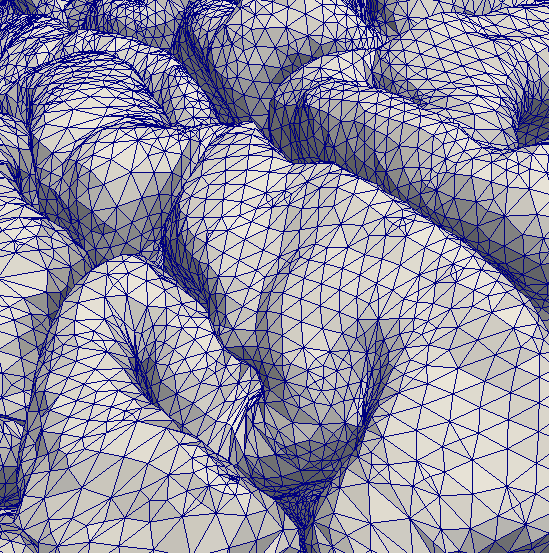
\includegraphics[width=0.49\textwidth]{./graphics/chp3/raw-stlmesh.png}
  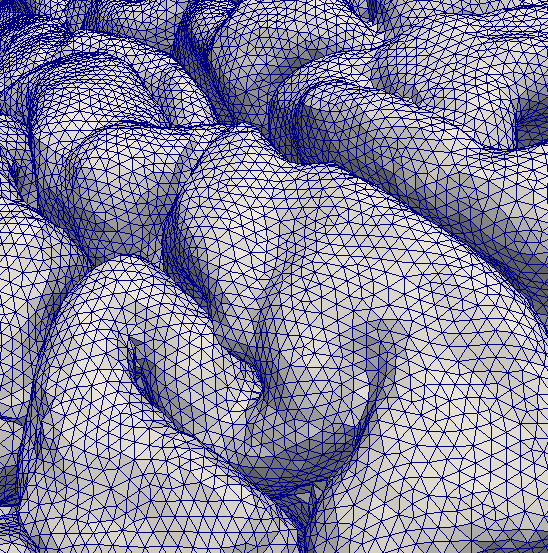
\includegraphics[width=0.49\textwidth]{./graphics/chp3/remesh-stlmesh.png}
  \caption{Original (left) pial surface and (right) after remeshing with \svmtk{}}
  \label{fig:chp3:ernie-remesh}
\end{figure}


\subsection{Smoothing a surface file}
\label{subsubsec:chp3:mesh-creation:smoothing}

To reduce the presence of non-physiological features such as sharp
corners, it may be advantageous to smoothen the surfaces prior to
volume meshing. \svmtk{} also includes utilities for smoothing surfaces, as
we demonstrate in the script below (included as
\emp{mri2fem/chp3/smooth\_surface.py} in the book scripts), using
our remeshed surface \emp{lh.pial.remesh.stl} as sample input.  It is worth 
noting that surface smoothing operations alter the position of existing 
vertices; in particular, smoothing does not alter the number of elements in 
the mesh.  %
%
\index{SVM-Tk!\emp{Surface}}
\index{smoothing}
%
Again, we define a short Python function
\pythoninline{smoothen\_surface} that can be called as
\newpythonsnippet{chp3}{smooth_surface.py}{19}{20}
\noindent The function itself reads
\newpythonsnippet{chp3}{smooth_surface.py}{0}{17}

The Boolean variable \pythoninline{preserve\_volume} determines
whether a shrinkage-preventing \cite{taubin1995curve} Taubin smoothing 
(\pythoninline{True}) or a Laplacian 
smoothing (\pythoninline{False}) process should be used.  From a conceptual
point of view, Taubin smoothing is essentially a local smoothing
iteration followed by a local `swelling' operation that aims to prevent 
any shrinkage in the volume of the original patch, whereas Laplacian smoothing 
consists only of local smoothing operations and the volume of the original
patch might not be preserved \cite{taubin1995curve}. Between the two, we
recommend Taubin smoothing. The integer value \pythoninline{n}
sets the number of times the smoothing process should take place. Higher
values will produce a smoother mesh; however, too high of a value may
result in a loss of resolution in brain features, such as the sulci and
gyri (grooves and bumps), on the brain surface. Finally, the floating
point value \pythoninline{eps} determines the strength of the
smoothing operation for each smoothing iteration, and should be in the
interval $[0, 1]$ with $0.0$ ($1.0$) indicating no (full)
smoothing.
\begin{figure}
  \centering
  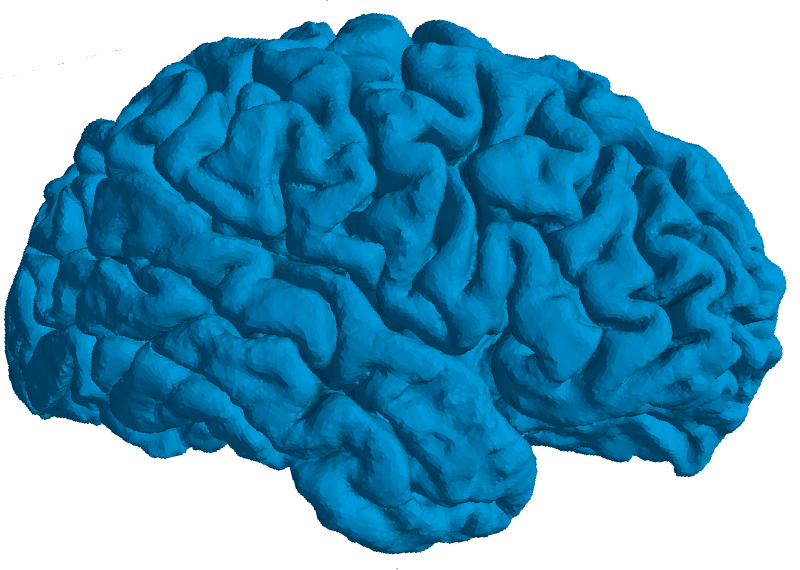
\includegraphics[width=0.30\textwidth]{./graphics/chp3/unsmoothed.png}
  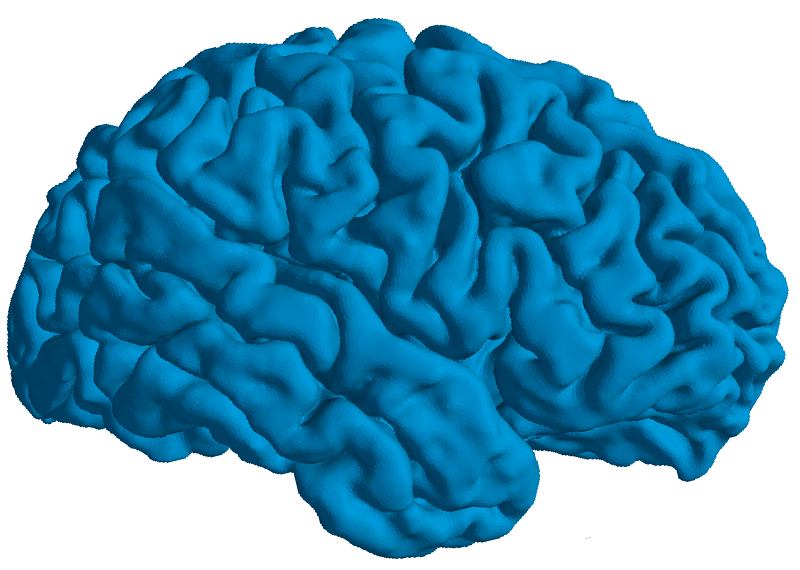
\includegraphics[width=0.30\textwidth]{./graphics/chp3/taubin-smoothed-10.png}
  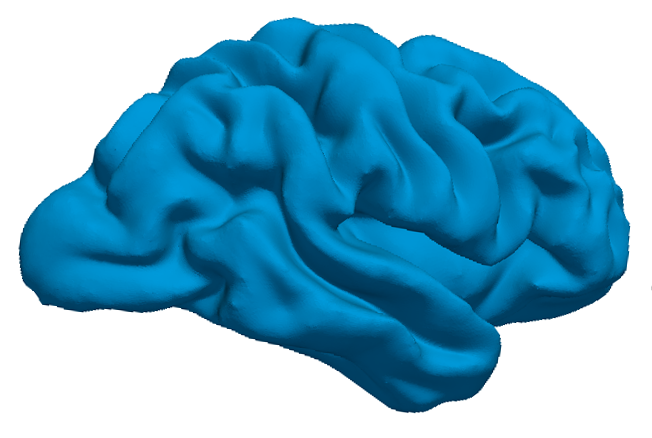
\includegraphics[width=0.30\textwidth]{./graphics/chp3/oversmoothing.png}
  \caption{Surface smoothing: original pial surface 
    (\emp{lh.pial.remesh.stl}, left), after Taubin smoothing with
    {\svmtk} (\emp{lh.pial.smooth.stl}, middle), and Laplacian over-smoothing (right).}
  \label{fig:chp3:ernie-smoothing}
\end{figure}
%
\index{ParaView}
\index{file format!STL}
\index{file format!mesh}

Figure~\ref{fig:chp3:ernie-smoothing} shows the result of 10
iterations of smoothing; over-smoothing of
the pial surface can lead to missing anatomical detail or errors
(for example Figure~\ref{fig:chp3:ernie-smoothing} (right)). It is generally 
advised to check the file visually by opening it directly, using either
ParaView or Gmsh, to determine if more or less smoothing is needed;
some surface STL files may require more or fewer iterations than
others.

We can generate a higher quality mesh in XML or XDMF format by
generating the volume mesh from the remeshed and smoothened STL
surface using the Python call
\begin{python}
create_volume_mesh("lh.pial.smooth.stl", "ernie.mesh")
\end{python}
followed by
\terminal{\$ meshio-convert ernie.mesh ernie.xml\\
\$ meshio-convert ernie.xml ernie.xdmf}
\noindent We will use the resulting \emp{ernie.xdmf} in the
simulations ahead in Chapter~\ref{sec:chp3:math}.

\subsection{Preventing surface intersections and missing facets}
\label{subsec:chp3:preventing-surface-intersections}

\svmtk{} also includes utilities for repairing surface faults:
\begin{itemize}
\item
  Surfaces constructed by FreeSurfer can have topological defects,
  such as missing facets.  Missing facets appear as `holes' in the surface, 
  i.e. a missing triangular simplex, when viewing a surface STL (.stl) file 
  using ParaView or Gmsh.  %holes. 
  %
  These defects can be repaired by following the
  FreeSurfer topological defects tutorial guide~\cite{freesurfer-wiki}.
  We can also attempt to fix missing surface facets using the \svmtk{}
  %However, we can also encounter surfaces with missing facets %,
  %that is, structural defects, which and 
  %that can be corrected with the \svmtk{}
  function \pythoninline{fill\_holes}.
\item
  The folds of pial surfaces can produce narrow gaps. Gaps that are
  shorter than the edges of the mesh may result in bridges instead
  of folds in the mesh, as exemplified in
  Figure~\ref{fig:chp3:juncture}. The function
  \pythoninline{separate\_narrow\_gaps} 
  identifies narrow gaps and uses an algorithm to separate them based on 
  the characteristics of the surrounding mesh.  The function requires a 
  negative value as input.  Lower values of $L$ results in a faster runtime for 
  for the algorithm, but may result in a more jagged surface.   
  Higher values of $L$, e.g.~those closer to zero, can extend computational 
  time but generally result in a smoother surface as a result.%
  %
  %
  %closes junctures until the edge distance between vertices is less
  %than the distance between unconnected vertices. The iterative
  %separation is performed by multiplying the outward surface normal
  %with a user-specified negative value. 
\item 
  The command \pythoninline{collapse\_edges} will combine short edges
  such that the new edge lengths are equal to the input target edge
  length.
\end{itemize}
\begin{figure}\sidecaption
  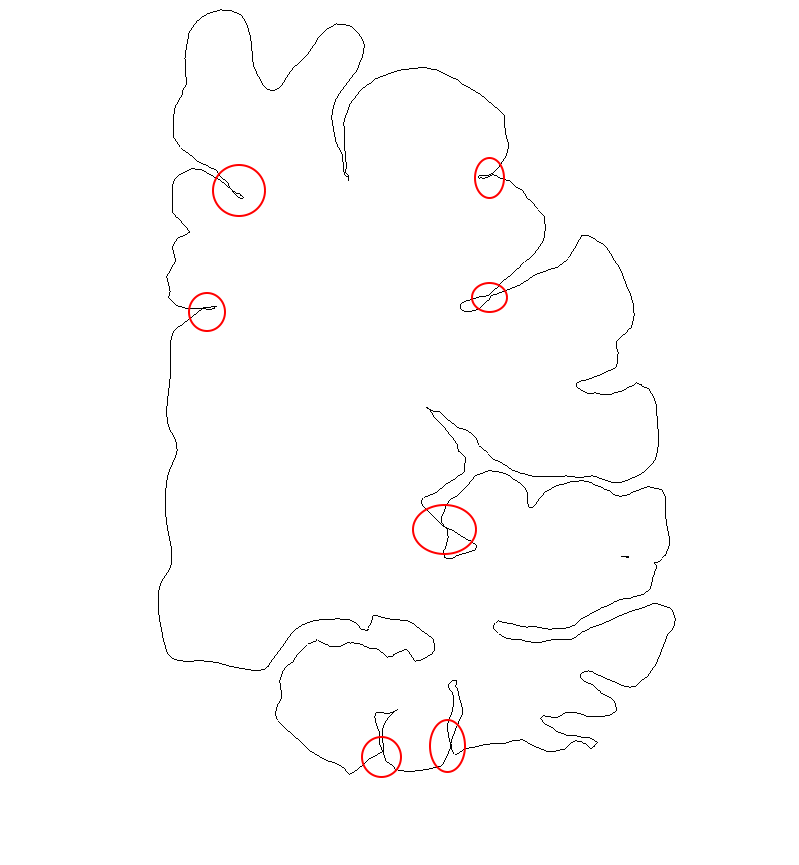
\includegraphics[width=0.5\textwidth]{./graphics/chp3/juncturers-gap.png}
  \caption{Illustration of close junctures in a coronal
    slice of the pial surface created by FreeSurfer.}
  \label{fig:chp3:juncture}
\end{figure}
%
\index{SVM-Tk}
\index{SVM-Tk!\emp{Surface}}
\index{repairing STL surfaces}
%
The following Python snippet illustrates the use of these commands
(included as \emp{mri2fem/chp3/svmtk\_repair\_utilities.py} in the
book scripts):
\newpythonsnippet{chp3}{svmtk_repair_utilities.py}{0}{11}
More commands involving multiple surfaces will be
covered in Chapter \ref{chp:chp4}.

\section{Simulation of diffusion into the brain hemisphere}
\label{sec:chp3:math}

With a mesh representing the domain of interest, we are ready to start
modeling and numerically simulating biophysical processes in this
domain. As a first example, we will study diffusion into the brain
parenchyma of a tracer injected in the subarachnoid space (SAS). This is a
setting encountered, for example, in clinical practice when gadobutrol is 
injected intrathecally (into the cerebrospinal fluid in the spinal
cord SAS)~\cite{ringstad2018brain}, and in experimental
research when fluorescent tracers such as dextran are injected in the
cisterna magna of mice~\cite{iliff2012paravascular,
  xie2013sleep}. Understanding the role of diffusion -- versus other
mechanisms, such as convection -- in the brain parenchyma is a topic of
substantial interest in physiology and medicine~\cite{abbott2018role}.

\subsection{Research question and model formulation}
\label{chp3:model}

Let us ask the following question: assuming that solutes move in the
brain parenchyma by diffusion alone, given an intrathecal injection of
the contrast agent gadobutrol as in glymphatic MRI
investigations~\cite{ringstad2018brain}, what would be the evolution
and distribution patterns of gadobutrol in the brain up to 24 hours
after injection?

To begin addressing this question, we define an initial boundary value
problem for the diffusion of gadobutrol in the brain parenchyma. To do
so, we need to prescribe the computational domain, initial conditions,
parameter values, and boundary conditions for \eqref{eq:diffusion}. It
is often a good idea to also think about the units when defining your
simulation scenario. In brain mechanics at the tissue or organ level,
millimeters (mm) or meters (m) and seconds (s) or minutes (min) are
often suitable choices of units, although we note of course that the
duration of some physiological processes is on the order of days,
months, or years.

Here, we let the concentration $u$ represent the (unit-less)
concentration, of gadobutrol tracer, solving~\eqref{eq:diffusion} in
$\Omega$. The image-based mesh of the left brain hemisphere (for
example \emp{ernie.xdmf}) defines the computational domain
$\Omega$. Formally, $\Omega$ is then the union of the cells in the
mesh. Note that the mesh defines the spatial coordinates of the domain
and consequently the spatial unit. Meshes generated from FreeSurfer
data are typically defined in terms of mm, and thus mm is the default
unit for the spatial scale. The spatial unit can be redefined by
rescaling the mesh, a simple operation in FEniCS. We also
pick a final time and time unit, for instance $T = 1440$ min ($T = 24$
hours).

We assume that no gadobutrol is present in the domain initially,
which translates to the initial condition
\begin{equation}
  \label{eq:chp3:ic}
  u_0(x, 0) = 0 \quad \text{ for all } x \in \Omega.
\end{equation}
Next, we assume that gadobutrol is instantaneously distributed to the brain 
surface via the CSF in the SAS by setting the
boundary condition:
\begin{equation}
  \label{eq:chp3:bc}
  u_d(x, t) = 2.813 \times 10^{-3} \quad x \in \partial \Omega, \quad t > 0
\end{equation}
where $\partial \Omega$ denotes the boundary of $\Omega$, which
represents the pial surface in this scenario. Assuming that the
concentration is known on the pial surface everywhere and at all times
is clearly a simplification. More realistic boundary conditions can
and have been considered in the
literature~\cite{croci2019uncertainty,valnes2020apparent}, and one
could also directly model the movement of tracer in the CSF in the
subarachnoid space~\cite{haga2017numerical,pizzichelli2017numerical}

Brain tissue is heterogeneous and anisotropic, which means that the
effective diffusion coefficient $D$ in~\eqref{eq:diffusion} should vary in
space (and probably in time over longer time scales) and be
tensor valued. We will address these aspects later in this book (in
Chapter~\ref{chap:dti}), but for now we just consider a uniform and
scalar-valued $D$. We estimate the
average effective diffusion coefficient of gadobutrol in brain tissue
to be
\begin{equation}
  D  
  = 4.32 \times 10^{-1} \, \text{mm$^2$/hour}
  = 7.2 \times 10^{-3} \, \text{mm$^2$/min}
\end{equation}
Finally, we assume that there are no sources or sinks of gadobutrol
within the brain parenchyma, and thus set
\begin{equation}
  f(x, t) = 0 \quad x \in \Omega, \quad t > 0.
\end{equation}
Again, this is clearly a simplification that does not account for
potential exit pathways for gadobutrol from the parenchyma.

\subsubsection{Quantities of interest}
The computed solution $u$ will vary in time and space and thus encodes
a substantial amount of information. We are often interested in, first,
merely inspecting the solution visually or qualitatively. For more
quantitative analysis and comparison with experimental or clinical
findings, we typically compute quantities of interest associated with
the solution. These quantities of interest can, for instance, be the
total volume of solute in the entire domain over time:
\begin{equation}
  \label{eq:chp3:qoi}
  Q(t) = \int_{\Omega} u (t) \dx, 
\end{equation}
the average concentration in local regions, or the concentration in
specific points $x$ over time: $u(x, t)$.

\subsection{Numerical solution of the diffusion equation}
\label{sec:chp3:model-problem-numerical-formulation}

%
\index{FEniCS}
%
To compute numerical solutions of the diffusion
equation~\eqref{eq:diffusion} in general, and our specific initial
boundary value problem in particular, we will use a finite difference
discretization in time and a finite element discretization in
space~\cite{langtangen2019introduction,
  gockenbach2006understanding}. This is a common approach and we will
implement this numerical scheme using FEniCS Project
software~\cite{logg2012automated,alnaes2015fenics,langtangen2016solving}. As
mentioned in our introductory remarks, we strongly encourage readers
unfamiliar with numerically solving partial differential equations
(PDEs) or FEniCS to study the FEniCS
tutorial~\cite{langtangen2016solving} before proceeding.

For the discretization in time, we define a set of discrete times $0 =
t_0 \leq t_1 \dots \leq t_N = T$, where $N$ is the number of time
steps and the time step (size) is $\tau_n = t_n - t_{n-1}$ for $n = 1,
\dots, N$. Our aim is to compute approximate solutions $u^n_h$
of~\eqref{eq:diffusion} such that $u^n_h \approx u(t_n)$ for each
$n$. To this end, we introduce the (first-order, backward) finite
difference approximation in time
\begin{equation}
  u(t_n) \approx u^n, \quad
  u_t(t_n) \approx \frac{1}{\tau_n} (u^n - u^{n-1}),
\end{equation}
and obtain the time-discrete equations for $n = 1, \dots, N$:
\begin{equation}
  \label{eq:chp3:time-discrete}
  \frac{1}{\tau_n} (u^n - u^{n-1}) - \Div D \Grad u^n = f(t_n) \quad \text{in } \Omega. 
\end{equation}

Next, for the finite element discretization in space, we derive a
discrete variational formulation of~\eqref{eq:chp3:time-discrete} by
multiplying it by test functions $\phi$ belonging to a finite element space $V$
defined relative to the mesh $\mesh$, integrating by parts, and moving
all known terms to the right-hand side to obtain the following fully
discrete problem: find the discrete solution $u_h^n \in V$ at each
time $n = 1, \dots, N$ such that
\begin{equation}
  \label{eq:chp3:discrete}
  \inner{u_h^n}{\phi} + \tau_n \inner{\Grad u_h^n}{\Grad \phi}
  =  \inner{u_h^{n-1}}{\phi} + \tau_n \inner{f^n}{\phi},  
\end{equation}
for all test functions $\phi \in V$, where we use the
$L^2(\Omega)$-inner product notation
\begin{equation}
  \inner{u}{\phi} = \int_{\Omega} u \, \phi \dx.
\end{equation}
In addition, we require the discrete solution to satisfy the
boundary condition~\eqref{eq:chp3:bc}, and to initially be given by the
initial condition~\eqref{eq:chp3:ic}.   

The fully discrete equation~\eqref{eq:chp3:discrete} is a good
starting point for the FEniCS implementation of this scheme. We choose
to approximate the solution using continuous piecewise linear finite
element spaces. 

\subsection{Implementation using {\fenics}}
\label{sec:chp3:fenics-code-implementation}

Our model problem is very similar to the heat equation problem
presented in the FEniCS tutorial~\cite[Chapter
  3.1]{langtangen2016solving}, and we base our implementation on the
algorithm and code presented there. We begin by importing the Python
module \pythoninline{fenics}, and we also import \pythoninline{numpy}
as a handy Python module for general numerics:
\newpythonsnippet{chp3}{diffusion.py}{0}{2}
%
\index{file format!XDMF}
\index{file format!h5}
%
\noindent We then read the mesh that we have just generated into the FEniCS
program. We use the XDMF mesh format and reader, since they are suitable for
large scale simulations and work seamlessly with MPI-parallel computing:
\newpythonsnippet{chp3}{diffusion.py}{4}{13}

\noindent We now define the parameters for the time discretization. We
choose to simulate up to 72 hours and choose a time step $\tau$
(\pythoninline{tau}) of three min. Note that we use the Constant type to
represent \pythoninline{time}; it is useful for updating functions
depending on time later. In addition, keeping track of the parameter units
used is good practice. Here we just use the comments, although much more
rigorous solutions, such as SymPy's unit
systems~\cite{meurer2017sympy}, could be used.
\newpythonsnippet{chp3}{diffusion.py}{15}{18}

\noindent We also define the diffusion coefficient, source function
and initial condition (even though the latter two are just zero):
\newpythonsnippet{chp3}{diffusion.py}{20}{25}

We now move on to consider the specification of the finite element
discretization. We first define the finite element space $V$ as the
Lagrange elements of degree 1 defined relative to our mesh, and then
define a \pythoninline{TrialFunction} and \pythoninline{TestFunction}
over this space 
\newpythonsnippet{chp3}{diffusion.py}{27}{30}

\noindent We next define a \pythoninline{Function} to hold the value
of the solution at the previous time step \pythoninline{u_}, and
initialize this function with the initial condition \pythoninline{u0}:
\newpythonsnippet{chp3}{diffusion.py}{32}{35}

\noindent Having defined these objects, we can express the variational
problem~\eqref{eq:chp3:discrete}, to be solved at each time step, in
code. We also redefine \pythoninline{u} as a
\pythoninline{Function} to represent the solution at the current time:
\newpythonsnippet{chp3}{diffusion.py}{37}{42}

\noindent Having defined the finite element space, we can also define
the boundary condition, which will be imposed on the linear system of
equations at each time step. 
\newpythonsnippet{chp3}{diffusion.py}{47}{51}
\noindent Note how we let the boundary value
\pythoninline{u_d} depend on the previously defined
\pythoninline{Constant} \pythoninline{time}. This way, when
\pythoninline{time} updates, so will \pythoninline{u_d} and
\pythoninline{bc}.

We have now defined all the elements of the model problem and
numerical method and can start stepping through the solution
algorithm. Since the bilinear form on the left hand side
of~\eqref{eq:chp3:discrete} does not vary in time, we can assemble
this matrix once, outside the time loop, for the sake of efficiency:  
\newpythonsnippet{chp3}{diffusion.py}{53}{55}
%
\index{ParaView}
%
In order to view our solutions using ParaView, we define a PVD file 
(indicated by the suffix \pythoninline{.pvd}) for 
%We define a PVD file (indicated by the suffix \pythoninline{.pvd}) for
storing the solution, computed at each time step, as well as the initial data. 
%in VTK format and
%store the initial solution. 
\newpythonsnippet{chp3}{diffusion.py}{57}{60}
\noindent %This is a file format convenient for visualization in
%ParaView. 
%Note that it is not a convenient format for reading the
%functions back into FEniCS however; for this purpose one should
%instead use the XDMF or h5 formats.
The PVD format is nice for visualization in ParaView but is not a convenient 
format for reading the functions back into FEniCS; for this purpose one should
instead use the XDMF or h5 formats.

Next, we compute the number of time steps, \pythoninline{N}, and initialize
NumPy arrays for storing computational quantities of interest at each
time step, such as the total amount of solute (\pythoninline{amounts})
cf.~\eqref{eq:chp3:qoi}, and the concentration (\pythoninline{concs})
at a specific point (\pythoninline{p}).
\newpythonsnippet{chp3}{diffusion.py}{62}{68}

Now we are ready to start stepping through time and to solve the finite
element system at each time step. We increment
\pythoninline{time} with the timestep~\pythoninline{tau}, assemble
the right hand side into the vector \pythoninline{b}, apply the
Dirichlet boundary condition, solve the resulting linear system using
an iterative solver (gmres, amg), and update the previous solution
with the current solution:
\newpythonsnippet{chp3}{diffusion.py}{70}{85} %
Note that the use of `gmres', in the solve function above, tells {\fenics} to 
use the `Generalized Minimal Residual Method' as the iterative solution 
technique; the use of `amg' specifies that the `Algebraic Multigrid Method' 
should be used as the preconditioning approach for the iterative method.  The 
interested reader can find more on the GMRES method, including convergence 
details, in \cite{greenbaum1997} while a review of algebraic multigrid 
is also available \cite{stuben2001}.  Both GMRES and AMG are well-suited to 
parabolic problems, like \eqref{eq:diffusion}, and {\fenics} supports several 
alternative iterative methods and preconditioning options 
\cite{langtangen2016solving} that can investigated if desired.  % 


We can compute the total amount of solute by integrating the concentration
over the domain, and the concentration in the specified point by
evaluating the computed solution at this point. We also store the
entire solution to the PVD file. Writing the solution to file can take
some time, and, for fine time steps, it may often be practical to 
do this only say every second, or 10th or 100th time step:
\newpythonsnippet{chp3}{diffusion.py}{87}{96}
It can also be practical to store the computed quantities in a file; reading 
the contents of the file, for plotting, at a later time:
\newpythonsnippet{chp3}{diffusion.py}{98}{101}

\index{plotting!matplotlib}
The Python module matplotlib offers quick and convenient plotting, and
we use this module to plot the quantities of interest (the total
amount of solute and the concentration at the given point) over time
and save these in, for instance, PNG format. The resulting plots are
shown in Figure~\ref{fig:chp3:png-plots}. The complete script
(including the plot code) is available in the book scripts
(\emp{mri2fem/chp3/diffusion.py}).  The concentration at various points can be 
investigated by modifying the value of $p$, in the script, as shown in the code 
block below:
\newpythonsnippet{chp3}{diffusion.py}{62}{68}

\begin{figure}
    \begin{tabular}{cc}
    \imagetop{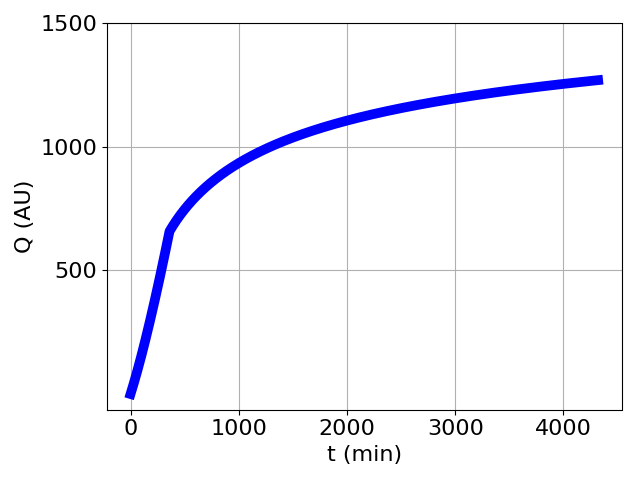
\includegraphics[width=0.49\textwidth]{./graphics/chp3/amounts.png}} &
    \imagetop{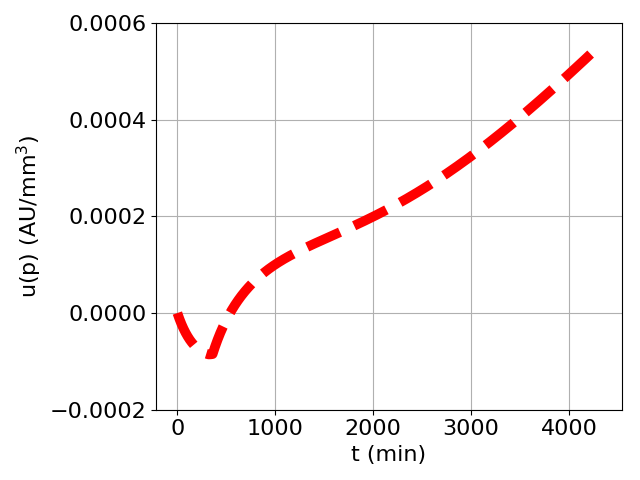
\includegraphics[width=0.49\textwidth]{./graphics/chp3/concentrations.png}}
    \end{tabular}
    \caption{Plots of the quantities of interest, in arbitrary units (AU), 
	associated with the computed concentration: total amount of solute 
	$Q$ over time $t$ (left) and concentration $u(p, t)$ for a given 
	point $p$ over time $t$ (right).}
    \label{fig:chp3:png-plots}
\end{figure}

\index{mass lumping}
The approximation of the solute concentration at a given point over
time demonstrates an interesting numerical artefact: the concentration
drops below zero to become negative at early times (between 0 and 550
min). Negative solute concentrations are clearly unphysiological, but
a common numerical problem with diffusion simulations. A partial and
often used remedy, including within the context of diffusion simulations
in the brain~\cite{croci2019uncertainty}, is \emph{mass lumping}. Mass
lumping can reduce spurious negative concentrations, but may worsen
the overall convergence of the numerical solutions. We will return
to this aspect in Chapter~\ref{chp:chp6}.

\subsection{Visualization of solution fields}
\index{ParaView}
To visualize computed solution fields, for instance, the
concentrations stored in u.pvd (and the associated u*.vtu files) in
the previous section, we will use ParaView. After launching the
ParaView graphical user interface (see
Chapter~\ref{sec:chp2:paraview}), we can open collections of files
by \button{File$\rightarrow$Open} and selecting the .pvd or .vtu
file(s) from the folder results. ParaView is a powerful and versatile 
visualization tool, and we refer the reader to the extensive resources 
available on the ParaView website~\cite{paraview:web} for guides, tutorials, 
and so forth. In Figure~\ref{fig:chp3:approximate-numerical-soln} below, we 
used ParaView to plot clips of snapshots of the solute
concentrations, with the x-axis as the normal direction for the clips
and the view direction, rescaled to the data range over all
  timesteps, and using the viridis color scheme.
\begin{figure}[h]
    \begin{tabular}{l l l l}
    \imagetop{2h}&  \imagetop{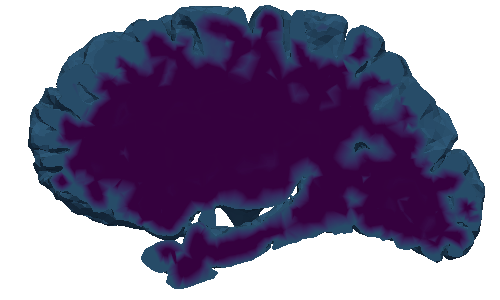
\includegraphics[width=0.4\textwidth]{./graphics/chp3/mri-tracer/2h}}&
    \imagetop{6h}&  \imagetop{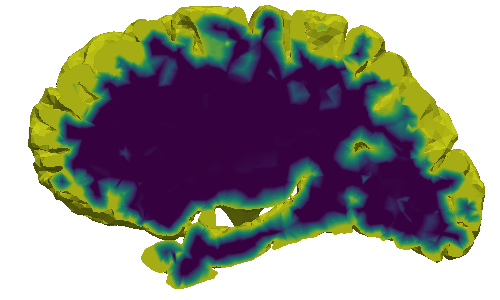
\includegraphics[width=0.4\textwidth]{./graphics/chp3/mri-tracer/6h}}\\
    \imagetop{12h}& \imagetop{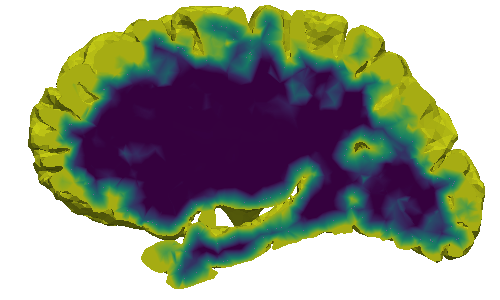
\includegraphics[width=0.4\textwidth]{./graphics/chp3/mri-tracer/12h}}&
    \imagetop{24h}& \imagetop{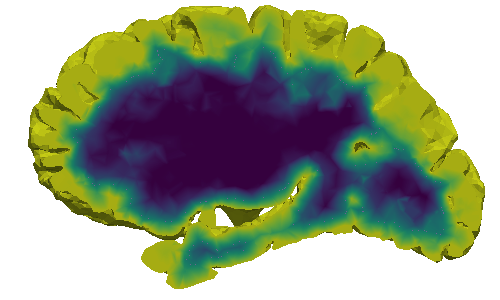
\includegraphics[width=0.4\textwidth]{./graphics/chp3/mri-tracer/24h}}\\
    \imagetop{48h}& \imagetop{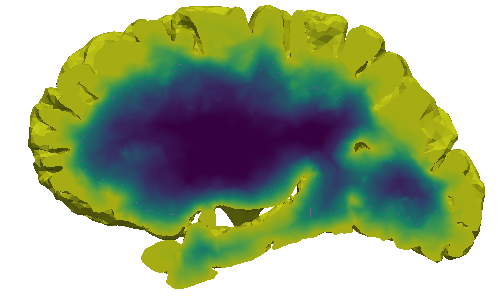
\includegraphics[width=0.4\textwidth]{./graphics/chp3/mri-tracer/48h}}&
    \imagetop{72h}& \imagetop{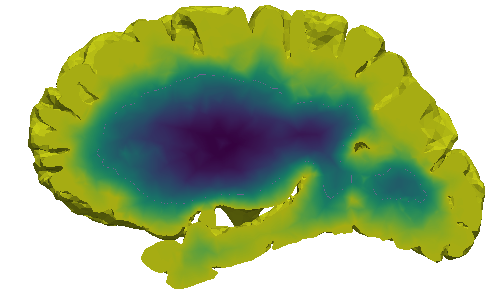
\includegraphics[width=0.4\textwidth]{./graphics/chp3/mri-tracer/72h}}
    \end{tabular}
    \caption{Simulated tracer concentration at given times (2, 6, 12, 24, 48, 
	and 72 hours) post-injection into subarachnoid CSF. Blue 
	represents lower values, while yellow represents higher values.  
	The scalar concentration is plotted on the whole brain volume mesh; the 
	mesh has been sliced, in ParaView, for sagittal visualization.}
    \label{fig:chp3:approximate-numerical-soln}
\end{figure}

\section{Advanced topics for working with larger cohorts}
\label{sec:chp3:advanced}
\index{DICOM}
We have now covered the entire computational pipeline from MR images
to numerical simulation and visualization for a single imaging
modality, a single stack of MRI data, and a single simulation scenario. In
this section, we will cover some more advanced topics useful for
working with more complex DICOM data collections.

\subsection{Scripting the extraction of MRI series}

When processing larger DICOM datasets consisting of a large number of
patients and/or studies, the extraction of single MRI series via a
graphical interface can become tedious and error-prone. An alternative
approach is to script the extraction of specific MRI series using
FreeSurfer command line utilities.

%
\index{FreeSurfer!\emp{mri\_probedicom}}
%
The extraction process consists of two command line steps: probing the
dataset for a given tag name and then extracting all data with the
given tag from the database. We will utilize the FreeSurfer command
\emp{mri\_probedicom} to examine and probe the DICOM metadata, so
ensure that FreeSurfer is installed and configured (see
Chapter~\ref{sec:chp2:tools:freesurfer}) before proceeding. The useful
command \emp{mri\_probedicom} can be used to compare the meta
data of different DICOM files with the flag \emp{-{}-compare} followed
by two DICOM filenames. We can also view the selected DICOM file by
using the flag \emp{-{}-view}, for example:
\terminal{\$ cd \erniedicom/DICOM \\
\$ mri\_probedicom -{}-i IM\_0162 -{}-view
}
\noindent To probe the book DICOM data set for the tag \textit{Protocol Name}, which
is associated with the numeric identifier 18 1030, issue the command
\terminal{\$ mri\_probedicom -{}-i IM\_0162 -{}-t 18 1030 \\
T13D
} 
\noindent The complete description of possible options to
\emp{mri\_probedicom} can be viewed by using the \emp{-{}-help} flag.

To extract files with a specific tag on the command-line, we can thus
probe each file, and copy files with a specific tag to a new
directory. This can be accomplished via, for example, the following bash script
(also available at \emp{mri2fem/chp3/mri\_sort.sh}). The script
takes three types of input, namely, the DICOM directory, the output directory and
an identifier for the protocol name:
\begin{lstlisting}[style=bashStyle]
#!/bin/bash
# 1st argument $1: input DICOM folder
# 2nd argument $2: the output copy directory
# 3rd argument $3: the identifier 

# Find all files in the directory and subdirectories
files=$(find $1 -type f ) 
for j in ${files}; do
    # Probe for protocol name (18 1030)
    name=$(mri_probedicom --i ${j} --t 18 1030) 

    # Check if identifier is part of protocol name.
    if [ "${name/$3}" != "$name" ]
       then
       # Copy file to (new) subdirectory 
       mkdir -p ${2}/${name//[[:blank:]]/}  
       cp ${j}  ${2}/${name//[[:blank:]]/} 
    fi
done
\end{lstlisting}

This script uses the bash command \emp{find} and the flag \emp{-type
  f} to find all files in the input directory and its
subdirectories. The script will go through all the files and probe
each file for the protocol name and check if the protocol name
contains the identifier argument. Each file with the identifier in the
protocol name will be copied to a folder named by the protocol name in
the output directory. Spaces are removed from the protocol name, which is preferred to avoid errors when using FreeSurfer.
Thus, we can use the script to extract all the images with the \emp{T1}
string in the protocol name from the sample data set:
\terminal{\$ cd \erniedicom \\
\$ ./mri\_sort.sh ./DICOM ./ "T1" }

\subsection{More about FreeSurfer's \emp{recon-all}}
\label{sec:chp3:advanced:recon-all}
%
\index{FreeSurfer!\emp{recon-all}}
%
The command \emp{recon-all} is the primary command for FreeSurfer,
since it will start the segmentation process. We have already
described the necessary flags for this command, but we will continue
the description with additional options. This description will be
on an introductory level. However, the interested reader can use the
flag \emp{-help}, which will print detailed information about the
entire process and provide references to related articles and texts.

The command \emp{recon-all} is a sequential process that consist of 34
different stages, divided into three different
steps~\cite{freesurfer-wiki}. Data will be produced throughout the
process, and are often required as input for the next stage. We can
initiate each step separately by using the following flags instead of
\emp{-all}.
% changed the autorecon-1 to autorecon1, etc in line with the freesurfer 
% documentation from https://surfer.nmr.mgh.harvard.edu/fswiki/recon-all
\begin{itemize}
\item \emp{-autorecon1}: starts the step-1 process, which includes stages 1 to 5, involving normalization and skull stripping; 
\item \emp{-autorecon2}: starts the step-2 process, which includes stages 6 to 23, involving segmentation and surface generation;
\item \emp{-autorecon2-pial}: starts the construction of the surfaces, which include stages 16 to 23, involving various surface operations;  
\item \emp{-autorecon3}: starts the step-3 process, which includes stages 24 to 34, involving statistical data generation and final parcellation;
\item \emp{-autorecon-all}: equivalent to \emp{-all}. 
\end{itemize} 

These flags can be useful for restarting the segmentation. For
instance, if a failure occurred at stage 36, then we can start over
from stage 24 rather than from the beginning by using the flag
\emp{-autorecon-3}. This approach can also be useful when it is
necessary to rerun the segmentation process after correcting an
error. In FreeSurfer, there exist two types of errors, known as hard
and soft errors. Hard errors will terminate the segmentation process,
while soft errors are errors that we find in the produced data. Soft
errors are mostly segmentation errors, such as the inclusion of the
dura in the segmentation and erroneous segmentation of white
matter. We can edit the segmentation to correct the error, and run
\emp{recon-all} with the flag \emp{-autorecon-2-pial}. This will
create new surfaces based on the corrected segmentation files. The
correction of soft errors will not be covered further in this
book. Instead, we refer to the FreeSurfer
documentation~\cite{freesurfer-wiki}.

%
\index{FreeSurfer}
\index{MRI!T2}
%
We continue with the flag \emp{-sd}, which can be used to specify the
subject directory for the \emp{recon-all} command. This can be quite
useful for separating the segmentation data for different
cohorts. The segmentation of CSF filled structures, such as the
ventricular system, may require the additional use of T2-weighted MR
images to obtain an acceptable quality. We can include T2 MRI with the
flag \emp{-{}-T2}, and we can use the flag \emp{-T2-pial} to use
the T2 MRI in the construction of pial surfaces.

The segmentation in FreeSurfer is based on the segmentation atlas of
healthy subjects; therefore, the segmentation can often encounter hard
errors for patients with abnormal brain anatomy. We can often allow
the segmentation to finish if we add the flag \emp{-notalairach},
which causes \emp{recon-all} to skip assertion points in the first step. The
log of \emp{recon-all} is documented in the folder \emp{scripts}
and all the specific command lines can be found in \emp{touch}.



